
\chapter{Giao thức CAN}

\section{Khái niệm}
CAN (Controller Area Network) là một giao thức truyền thông nối tiếp được phát triển bởi hãng Bosch vào những năm 1980 để giải quyết nhu cầu trao đổi dữ liệu giữa các thiết bị điện tử trong xe ô tô. Trước khi có CAN, các hệ thống điều khiển trong xe phải kết nối trực tiếp với nhau bằng dây dẫn, gây tốn kém và khó bảo trì. Việc sử dụng CAN cho phép các bộ điều khiển (ECU) chia sẻ dữ liệu với nhau thông qua một đường truyền chung, từ đó giảm thiểu số lượng dây, tăng độ tin cậy và khả năng mở rộng hệ thống.

Giao thức CAN hiện được chuẩn hóa trong tiêu chuẩn ISO 11898 và đã vượt ra khỏi ngành công nghiệp ô tô, được ứng dụng rộng rãi trong công nghiệp tự động hoá, robot, y tế, hàng không và các hệ thống nhúng.

\subsection{Sơ đồ cấu trúc mạng CAN}
Dưới đây là sơ đồ kết nối tổng quát giữa các Node thông qua bộ điều khiển (CAN Controller) và bộ thu phát (CAN Transceiver) trên đường truyền vật lý:

\begin{figure}[H]
	\centering
	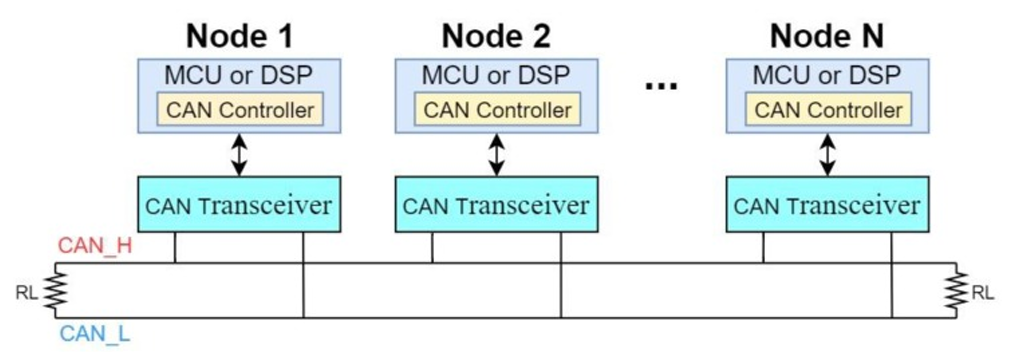
\includegraphics[width=1\textwidth]{images/CAN.png}
	\caption{Mạng CAN tổng quát}
\end{figure}

\subsection{Đặc điểm nổi bật của giao thức CAN}
\begin{itemize}[leftmargin=*]
    \item \textbf{Hoạt động theo mô hình đa master (multi-master):} Mọi thiết bị (node) trên mạng đều có quyền khởi tạo truyền dữ liệu. Điều này giúp mạng CAN linh hoạt hơn so với các mô hình truyền thống chỉ có một master điều khiển.
    \item \textbf{Truyền thông không định địa chỉ thiết bị:} Khác với giao thức UART hoặc I2C, CAN không dùng địa chỉ thiết bị. Thay vào đó, mỗi khung dữ liệu mang một ID (identifier) đại diện cho nội dung thông điệp. Các node sẽ lọc và xử lý dữ liệu theo ID mà chúng quan tâm. Điều này giúp tăng tính linh hoạt và khả năng mở rộng hệ thống.
    \item \textbf{Cơ chế ưu tiên truyền:} Trong trường hợp nhiều node cùng muốn truyền dữ liệu, giao thức CAN sẽ so sánh ID theo bit từng bước để quyết định thiết bị nào được phép tiếp tục truyền. ID có giá trị nhị phân thấp hơn (ưu tiên cao hơn) sẽ giành quyền truy cập bus. Quá trình này gọi là arbitration và diễn ra hoàn toàn tự động mà không gây xung đột.
    \item \textbf{Phát hiện và xử lý lỗi mạnh mẽ:} CAN có nhiều cơ chế phát hiện lỗi như:
    \begin{itemize}
        \item \textit{Bit monitoring:} Kiểm tra sự khác biệt giữa bit gửi và nhận.
        \item \textit{CRC check:} Kiểm tra tính toàn vẹn khung dữ liệu.
        \item \textit{ACK check:} Đảm bảo dữ liệu được ít nhất một node khác nhận thành công.
        \item \textit{Form check:} Kiểm tra định dạng của khung dữ liệu.
    \end{itemize}
    Nếu phát hiện lỗi, node sẽ tự động phát một Error Frame và yêu cầu gửi lại.
    \item \textbf{Tốc độ truyền dữ liệu linh hoạt:} Giao thức CAN hỗ trợ nhiều tốc độ khác nhau tùy theo chiều dài đường truyền. Trên thực tế:
    \begin{itemize}
        \item Với khoảng cách ngắn (dưới 40m), có thể đạt tốc độ tối đa 1 Mbps.
        \item Với khoảng cách dài (lên đến 1 km), tốc độ có thể giảm xuống khoảng 50 kbps.
    \end{itemize}
    Điều này làm cho CAN phù hợp với cả hệ thống nhỏ lẫn hệ thống phân tán rộng.
    \item \textbf{Giao tiếp đồng bộ và thời gian thực:} CAN sử dụng chuẩn mã hóa NRZ (Non-Return to Zero) và kỹ thuật bit stuffing để đồng bộ hóa giữa các node mà không cần xung clock ngoài. Điều này giúp đảm bảo giao tiếp thời gian thực, đặc biệt quan trọng trong các hệ thống an toàn như phanh ABS, điều khiển động cơ hay túi khí.
    \item \textbf{Chi phí thấp, độ tin cậy cao:} Nhờ vào khả năng xử lý lỗi, giảm thiểu dây nối và chi phí phần cứng, CAN trở thành lựa chọn hàng đầu cho các hệ thống nhúng cần độ tin cậy cao với chi phí hợp lý.
\end{itemize}

\section{Nguyên tắc hoạt động}

\subsection{Cấu trúc khung dữ liệu (Data Frame)}
\begin{table}[h!]
\centering
\begin{tabularx}{\textwidth}{l X}
\toprule
\textbf{Trường} & \textbf{Vai trò} \\
\midrule
Start of Frame & Xác định bắt đầu một khung dữ liệu. \\
Arbitration Field & Chứa ID và bit RTR (Remote Transmission Request). \\
Control Field & Xác định độ dài dữ liệu. \\
Data Field & Dữ liệu truyền đi (từ 0 đến 8 byte). \\
CRC Field & Dùng để kiểm tra lỗi dữ liệu truyền. \\
ACK Field & Thiết bị nhận phản hồi xác nhận khung hợp lệ. \\
End of Frame & Đánh dấu kết thúc khung dữ liệu. \\
\bottomrule
\end{tabularx}
\caption{Cấu trúc chi tiết các trường trong Data Frame}
\end{table}

\subsection{Phân loại ID}
Trong giao thức CAN, mỗi khung dữ liệu mang một mã định danh (ID - Identifier) thay vì địa chỉ thiết bị. ID được sử dụng để xác định nội dung thông điệp, phân mức ưu tiên trong quá trình tranh chấp truyền (arbitration) và giúp các node lọc dữ liệu cần thiết.

\begin{itemize}[leftmargin=*]
    \item \textbf{Standard ID (11 bit):}
    Là định dạng gốc của chuẩn CAN theo ISO 11898-1, còn gọi là Base Frame Format. Định dạng này gồm 11 bit, cho phép tối đa $2^{11} = 2048$ mã định danh khác nhau. Thường được sử dụng rộng rãi trong các hệ thống nhỏ, số lượng thiết bị hoặc thông điệp ít. Khung dữ liệu ngắn giúp giảm thời gian truyền, tăng hiệu quả mạng.
    
   quát\begin{figure}[H]
   	\centering
   	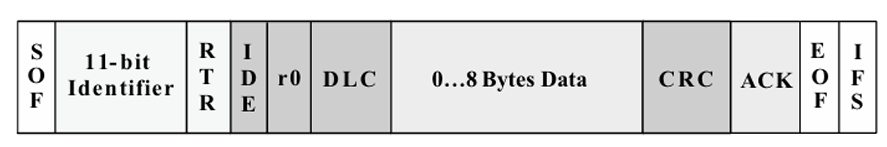
\includegraphics[width=1\textwidth]{images/CAN_ID.png}
   	\caption{Standard CAN: 11-Bit Indentifier}
   \end{figure}

    \item \textbf{Extended ID (29 bit):}
    Mở rộng từ chuẩn CAN cơ bản để đáp ứng nhu cầu phức tạp hơn. Cấu trúc gồm 11 bit gốc + 18 bit mở rộng, tổng cộng 29 bit. Định dạng này cho phép tối đa $2^{29} \approx 537$ triệu mã định danh khác nhau. Thường dùng trong các hệ thống lớn như xe hiện đại, hệ thống công nghiệp quy mô lớn. Hệ thống phân biệt bằng bit điều khiển IDE (Identifier Extension): nếu $\text{IDE} = 1 \Rightarrow$ sử dụng Extended ID.
    
    \begin{figure}[H]
    	\centering
    	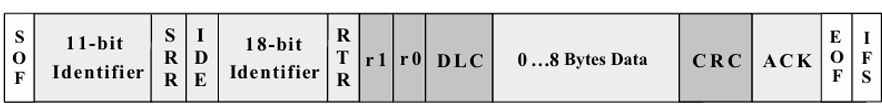
\includegraphics[width=1\textwidth]{images/CAN_EX.png}
    	\caption{Extended CAN: 29-Bit Indentifier}
    \end{figure}
\end{itemize}

\subsection{Truyền và nhận dữ liệu}
\begin{itemize}
    \item Tất cả thiết bị đều giám sát liên tục bus CAN.
    \item Thiết bị bắt đầu truyền khi phát hiện bus rảnh.
    \item Cơ chế arbitration dựa vào ID: thiết bị có ID nhỏ hơn sẽ được ưu tiên.
    \item Sử dụng mã hóa NRZ và kỹ thuật bit stuffing để đảm bảo đồng bộ.
\end{itemize}

\subsection{Phát hiện lỗi}
\begin{itemize}
    \item \textbf{Bit Monitoring:} So sánh bit truyền và bit nhận trên bus.
    \item \textbf{CRC Checking:} Kiểm tra tính toàn vẹn của dữ liệu.
    \item \textbf{Form Checking:} Đảm bảo khung dữ liệu đúng định dạng.
    \item \textbf{ACK Checking:} Thiết bị nhận phải xác nhận bằng cách gửi ACK.
\end{itemize}

\section{Ứng dụng trong Automotive: Hệ thống ô tô}
Trong các phương tiện giao thông hiện đại, đặc biệt là ô tô, giao thức CAN đóng vai trò là xương sống trong mạng truyền thông nội bộ. Với khả năng truyền thông tin hiệu quả, đáng tin cậy và chi phí thấp, CAN đã trở thành tiêu chuẩn công nghiệp trong các hệ thống điện tử trên xe.

\subsection{Các hệ thống tiêu biểu sử dụng giao thức CAN}
\begin{itemize}
    \item \textbf{ECU động cơ (Engine Control Unit):} Điều khiển hoạt động của động cơ như phun nhiên liệu, đánh lửa, kiểm soát khí xả, v.v.
    \item \textbf{Hệ thống túi khí (Airbag System):} Giao tiếp giữa các cảm biến va chạm, bộ xử lý và bộ kích hoạt túi khí để đảm bảo phản ứng tức thời khi xảy ra va chạm.
    \item \textbf{Hệ thống phanh ABS/ESP:} Trao đổi dữ liệu liên tục giữa cảm biến tốc độ bánh xe, ECU phanh và các mô-đun ổn định thân xe để ngăn trượt và lật xe.
    \item \textbf{Hệ thống điều khiển tiện nghi:} Bao gồm điều hòa không khí, điều chỉnh ghế, gương, cửa sổ, đèn nội thất, thường kết nối qua mạng CAN tốc độ thấp (Low-Speed CAN).
    \item \textbf{Màn hình thông tin và giải trí (Infotainment):} Kết nối giữa bảng điều khiển trung tâm, màn hình, bộ định vị GPS, hệ thống âm thanh, và các nút điều khiển trên vô lăng.
\end{itemize}

\subsection{Phân tầng mạng CAN trong ô tô}
Trong thực tế, các hệ thống điện tử trong xe thường được chia thành các tầng mạng CAN khác nhau, tùy vào tốc độ và mức độ quan trọng:
\begin{itemize}
    \item \textbf{High-Speed CAN (500 kbps - 1 Mbps):} Dùng cho các hệ thống an toàn và điều khiển động cơ, yêu cầu tốc độ cao và phản hồi nhanh.
    \item \textbf{Low-Speed / Fault-Tolerant CAN (125 kbps):} Dùng cho các chức năng thân xe như đèn, gương, khóa cửa, nơi yêu cầu tốc độ không quá cao nhưng độ ổn định quan trọng.
    \item \textbf{CAN FD (Flexible Data-rate):} Được tích hợp trong các xe mới để truyền lượng dữ liệu lớn hơn (như từ camera, radar) với tốc độ cao hơn và độ trễ thấp hơn.
\end{itemize}

